\chapter{Total Internal Reflection}\label{lec:lec32}

\begin{mdframed}[backgroundcolor=lightblue, linewidth=1pt, hidealllines=true]
\section{Objectives}
\begin{enumerate}[(i)]
\item Understand the conditions and implications of total internal reflection.
\item Analyze reflection coefficients and their relevance in different polarizations during total internal reflection.
\item Explain the behavior of fields in medium 2 and their role in total internal reflection.
\item Define reactive fields and their significance in the context of power flow during total internal reflection.
\item Describe the relationship between total internal reflection and guiding electromagnetic energy in wave guides.
\end{enumerate}
\end{mdframed}

\section{Introduction}

In this chapter, we will discuss a special case of reflection across a dielectric boundary\index{dielectric boundary} called Total Internal Reflection. We studied total internal reflection at the high school level where it was understood that, if a ray is incident at an angle greater than the critical angle\index{critical angle}, the ray is completely reflected back into the same medium. However, this understanding is a rather superficial one. Here we do a detailed study of the phenomenon of TOTAL INTERNAL REFLECTION\index{total internal reflection}.

\section{Snell's Law}
From Snell's Law,
\begin{align}
\beta_1 \sin\theta_i = \beta_2 \sin\theta_t
\label{eqn:eqn32_1}
\end{align}
where $\beta_1 and \beta_2$ are the phase constants in the two media. Recall;
$$ \beta_{1} = \omega\sqrt{\mu_{1}\epsilon_{1}}$$
$$ \beta_{2} = \omega\sqrt{\mu_{2}\epsilon_{2}}$$
\begin{align*}
\omega\sqrt{\mu_1\epsilon_{1}} \sin\theta_i &= \omega\sqrt{\mu_2\epsilon_2}  \sin\theta_t\\
&\text{or}\\
\sqrt{\mu_1\epsilon_{1}} \sin\theta_i &= \sqrt{\mu_2\epsilon_2}  \sin\theta_t
\end{align*}
If the medium parameters are such that,
\begin{align}
\frac{\beta_1}{\beta_2}\sin\theta_i > 1
\end{align}
Then there is no wave nature in medium 2 for which the angle $\sin\theta_t$ can propagate. It is more of an imaginary angle which lacks direction. And even though phase conditions in equation~\ref{eqn:eqn32_1} is satisfied, there is no physical angle $\theta_t$ for which
\begin{align}
\sin\theta_t > 1
\label{eqn:eqn32_3}
\end{align}
This poses a very interesting case. Now we require in our reflection co-efficient expression that the quantity
\begin{align}
\cos\theta_t = \sqrt{1-\sin^2\theta_t}
\end{align}
Substituting the expression for $\sin^{2}\theta_{t}$,
\begin{align*}
\cos\theta_t = \sqrt{1-(\frac{\beta_1}{\beta_2}\sin\theta_i)^2}
\end{align*}
this leaves the quantity $1 - (\frac{\beta_1}{\beta_2}\sin\theta_i)^2$ always negative and thus, the quantity $\sqrt{1 - (\frac{\beta_1}{\beta_2}\sin\theta_i)^2}$ imaginary. So we make it positive to satisfy the medium parameter in which $\frac{\beta_1}{\beta_2}\sin\theta_i > 1$
\begin{align}
\cos\theta_t = j\sqrt{(\frac{\beta_1}{\beta_2}\sin\theta_i)^2-1}
\label{eqn:eqn32_5}
\end{align}
Now again, we see that from equation~\ref{eqn:eqn32_3} and equation~\ref{eqn:eqn32_5} 
that there is no physical angle $\theta_t$ for which the wave would be propagated.

However for the angle $\theta_t$ and $\theta_i$ we would still have reflection and transmission coefficients, so we go back and substitute $\cos\theta_t$ in the reflection co-efficient expression.

Recall we had two cases of reflection coefficients.
\begin{align*}
\end{align*}For the Perpendicular case:
\begin{equation}
\Gamma_\perp\ = \frac{\eta_2\cos\theta_i - \eta_1\cos\theta_t}{\eta_2\cos\theta_i + \eta_1\cos\theta_t}
\label{eqn:eqn32_6}
\end{equation}

For the Parallel case:
\begin{equation}
\Gamma_\parallel = \frac{\eta_1\cos\theta_i - \eta_2\cos\theta_t}{\eta_1\cos\theta_i + \eta_2\cos\theta_t}
\label{eqn:eqn32_7}
\end{equation}
Note: $\eta_1$ and $\eta_2$ are interchanged for both cases otherwise they are similar. 

substituting equation~\ref{eqn:eqn32_5} in equation~\ref{eqn:eqn32_7},
\begin{align}
\Gamma_\parallel = \frac{\eta_1\cos\theta_i - j\eta_2\sqrt{(\frac{\beta_1}{\beta_2}\sin\theta_i)^2-1}}{\eta_1\cos\theta_i + j\eta_2\sqrt{(\frac{\beta_1}{\beta_2}\sin\theta_i)^2-1}}
\label{eqn:eqn32_8}
\end{align}
Note: we would get the same expression for the perpendicular polarization case but with $\eta_1$ and $\eta_2$ interchanged. 

What's important to note here is that the expression in equation~\ref{eqn:eqn32_8} is of the form
\begin{equation}
\frac{a - j b}{a + j b}
\end{equation}
and as we know, expressions of the form always have a magnitude equal  to 1 at an angle $\angle-2\tan^-{1}(\frac{b}{a})$ that is:
\begin{equation}
\frac{a - j b}{a + j b} = 1\angle - 2\tan^{-1}(\frac{b}{a})
\end{equation} 
And since the modulus(or magnitude) of the reflection coefficient is 1, whatever power is incident on the media interface is totally reflected.
So in this case, even though we have a dielectric boundary, the entire power is reflected back into medium 1 with a phase change given by $\angle-2\tan^-{1}(\frac{b}{a})$ and no power is transmitted into medium 2. Hence, this phenomenon is referred to as \textbf{Total internal reflection}.

\section{Conditions For Total Internal Reflection}
\begin{enumerate}[(i)]
\item For total internal reflection to occur, then the condition below has to be satisfied.
\begin{equation*}
\frac{\beta_1}{\beta_2}\sin\theta_i > 1
\end{equation*}
in terms of medium parameters
\begin{equation*}
\frac{\sqrt{\mu_1\epsilon_1}}{\sqrt{\mu_2\epsilon_2}}\sin\theta_i > 1
\end{equation*}
$\theta_i$ can attain a maximum value of $90^{o}$, therefore the maximum value of $\sin\theta_i$ = $\sin$90 = 1, this means, for the above condition to be meant,
\begin{equation}
\sqrt{\mu_1\epsilon_1} > \sqrt{\mu_2\epsilon_2}
\end{equation}
So if $\sqrt{\mu_1\epsilon_1} > \sqrt{\mu_2\epsilon_2}$, then there is a possibility of total internal reflection.

$\sqrt{\mu_1\epsilon_1} > \sqrt{\mu_2\epsilon_2}$ implies that medium 1 is a denser medium compared to medium 2. So essentially, when the wave goes from a denser medium to a less dense medium, then there is a possibility of total internal reflection.

For a pure dielectric(or non magnetic material) where, $\mu_1$ and $\mu_2$ are equal,
\begin{equation*}
\sqrt{\epsilon_1} > \sqrt{\epsilon_2}
\end{equation*}
Recall, refractive index, $n = \sqrt{\epsilon}$, thus
\begin{align*}
n_1 > n_2
\end{align*}
Where $n_1$ and $n_2$ are the refractive indexes of medium 1 and medium 2 respectively.

Now the angle at which $\sin\theta_t = 1$ is called the CRITICAL ANGLE\index{critical angle}, beyond which if an incident wave is launched, there would be no transmitted wave in the second medium.

This phenomenon is shown in Figure~\ref {critical_angle}.
\begin{figure}[h]
\centering
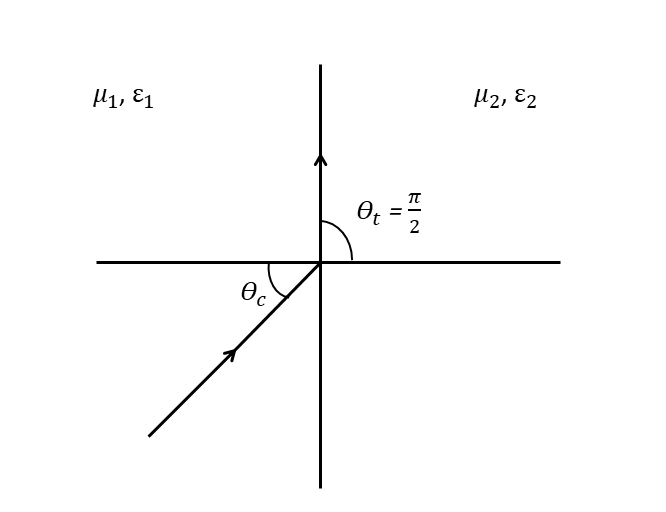
\includegraphics[width=1\linewidth]{\pathtopartone/graphics/critical_angle}
\caption{Critical angle}
\label{critical_angle}
\end{figure}

\begin{equation*}
\sqrt{\mu_1\epsilon_1} \sin\theta_c = \sqrt{\mu_2\epsilon_2}
\end{equation*}
similarly for pure dielectric media, 
\begin{align*}
n_1 \sin\theta_c = n_2
\end{align*}
Or the critical angle
\begin{align*}
\theta_c = \sin^{-1}(\frac{n_2}{n_1}) 
\end{align*}
Now what we have not discussed, however, is that, when the total internal reflection takes place, the wave which is reflected, undergoes a phase change at the interface. This phase change is a function of the medium parameters and the angle of incidence. So in general, we can say that by choosing appropriate parameters for the media, and the angle of incidence, we can generate an arbitrary phase difference between the incidence and the reflected wave. This would happen for both parallel and perpendicular polarization. However, the parallel and perpendicular polarization have $\eta_1$ and $\eta_2$
interchanged between them. So a and b in $\frac{a - j b}{b + j b}$ are different for parallel and perpendicular polarizations. This means that the phase changes which the wave undergoes for the two polarizations are different.

\item The wave undergoes a phase change at Total Internal Reflection the phase change is different for parallel and perpendicular polarizations.

If we write out explicitly, the phase changes for parallel and perpendicular polarization, we have;
\begin{equation}
\phi_\parallel = -2\tan^{-1}\frac{\eta_2\sqrt{(\frac{\beta_1}{\beta_2}\sin\theta_i)^2-1}}{\eta_1\cos\theta_i}
\end{equation}
\begin{equation}
\phi_\perp = -2\tan^{-1}\frac{\eta_1\sqrt{(\frac{\beta_1}{\beta_2}\sin\theta_i)^2-1}}{\eta_2\cos\theta_i}
\end{equation}
From here we see that the two polarizations do not undergo the same phase change. But later we'll see the implication of the phase change for the different kinds of polarization when Total Internal Reflection takes place in the dielectric boundary. 

\item For fields in medium 2

Recall:

The phase expression for a transmitted wave in medium 2 is
\begin{equation*}
\bar{E}_t = E_{t}e^{-j \beta_2(x\sin\theta_t + z\cos\theta_t)}
\end{equation*}
From Snell's Law and keeping phase gradient same $\bar{E}_t$ is written out explicitly as:
\begin{align}
\bar{E}_t = E_te^{- j x\beta_2\sin\theta_t - j z\beta_2\cos\theta_t}
\end{align}
substituting for $\cos\theta_t$ from equation~\ref{eqn:eqn32_5}
and $\sin\theta_t$ from equation~\ref{eqn:eqn32_1}
\begin{equation*}
\bar{E}_t = E_te^{- {j x\beta_1\sin\theta_i}  -  z \beta_2\sqrt{{(\frac{\beta_1}{\beta_2}\sin\theta_i)}^2 - 1}}
\end{equation*}
\begin{equation}
\bar{E}_t = E_te^{- {j x\beta_1\sin\theta_i}  -  z \sqrt{{(\beta_1\sin\theta_i)}^2 - \beta_{2}^{2}}}
\end{equation}
From the above equation,

The amplitude term is:
\begin{equation}
e^{-z\sqrt{\beta_1^2\sin^2\theta_i - \beta_2^{2}}}
\label{eqn:amplitude_term_total_internal_reflection}
\end{equation}
and the phase term:
\begin{equation}
e^{- j x\beta_1\sin\theta_i}
\label{eqn:phase_term_total_internal_reflection}
\end{equation}
From these equations, we see the field is exponentially dying down as a function of z and the phase varies as a function of x in medium 2.
\end{enumerate}
Now with total internal reflection, the travelling wave nature is only in the x-direction as the phase variation only occurs in the x-direction. So the fields are no longer travelling in the z-direction.

Essentially, equation~\ref{eqn:amplitude_term_total_internal_reflection} gives decaying fields in the z direction and equation~\ref{eqn:phase_term_total_internal_reflection}  gives a travelling wave in the x direction. This is depicted in figure~\ref{fig:amplitude_decay_total_internal_reflection}
\begin{figure}[h]
\centering
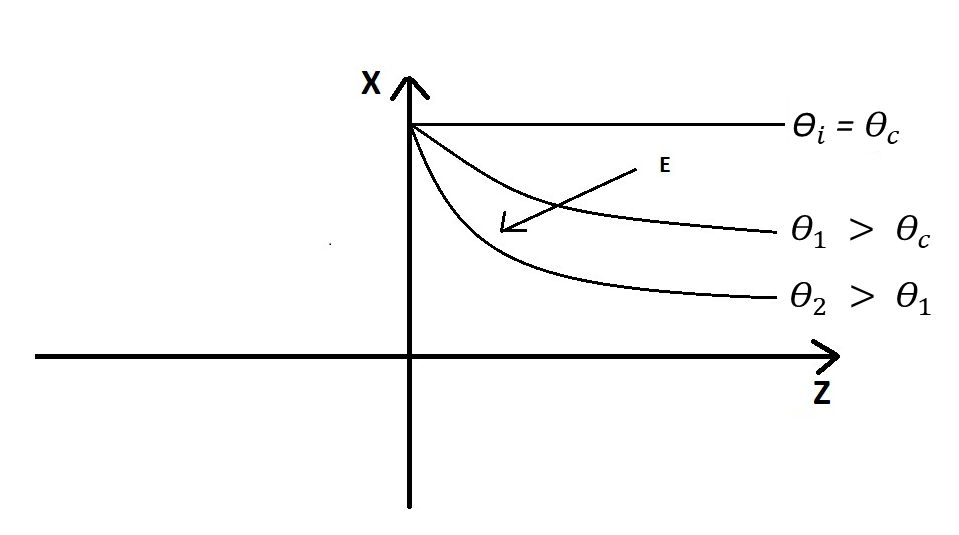
\includegraphics[width=1\linewidth]{\pathtopartone/graphics/amplitude_decay}
\caption{Amplitude decay of fields in medium 2}
\label{fig:amplitude_decay_total_internal_reflection}
\end{figure}

At angle $\theta_i = $ $\theta_c$, the term $e^{-z\sqrt{\beta_1^2\sin^2\theta_i - \beta_2^{2}}}$ reduces to $1$ so the amplitude of the field remains constant. Hence the field does not decay in medium 2. However, as $\theta_{i}$ increases more and more beyond $\theta_{c}$, the decay becomes faster as shown in figure~\ref{fig:amplitude_decay_total_internal_reflection}. 
So at the critical angle, the field essentially extends up to infinity at a constant amplitude and as the angle of incidence increases more and more beyond the critical angle, the field gets more and more confined towards the dielectric interface. The important observation is that the field never goes to zero in medium 2 under any condition. The field is always non-zero in medium 2. Theoretically, no matter how small this amplitude is, it will extend up to infinity in the z-direction as it gets closer and closer to zero but never reaches zero.
So when total internal reflection takes place at the media interface, from what we learnt in high school, it was like the total power got reflected in medium 1 and nothing existed in medium 2. There was no discussion at all as to what was the behaviour of the fields in medium 2 or the role medium 2 needed to play in total internal reflection. Once we had the critical condition for total internal reflection satisfied, we didn't bother about the point beyond the boundary into medium 2. But now we understand that we cannot ignore the region of medium 2 beyond the boundary. The fields have to exist in the form shown in medium 2 for total internal reflection to take place, and they are as important as the fields in medium 1. The fields in medium 2 are required for us to satisfy the continuity equation at the boundary. It is these fields in medium 2 that support the total internal reflection phenomenon. If any disturbance is created to these fields in medium 2, then the total internal reflection phenomenon is also disturbed and we cannot have a total internal reflection. So to have a good total internal reflection phenomenon, we must have the field in medium 2 as confined to the interface as much as possible. That means we must launch a wave with an angle larger than the critical angle for as much as possible so that the field dies down rapidly in medium 2 as fast as possible and thus confined to a thickness z in medium 2 that is extremely small.

Secondly, we must provide a certain region from the dielectric interface in medium 2 of a thickness where the fields in medium 2 are protected. If these two conditions are guaranteed, then we will have a total internal reflection phenomenon. Theoretically, unless we provide an infinite region in medium 2, and the fields properly protected, then we cannot have an ideal total internal reflection phenomenon.

\section{Reactive Fields}

We conclude that when total internal reflection takes place, the fields in medium 2 exist, and the transmission coefficient is not zero. When the total power is reflected, $|\Gamma| = 1$ but this doesn't mean that the transmission coefficient is zero because the transmission coefficient doesn't always mean that there is a power flow in medium 2. So as we have seen, the fields which are dying down in medium 2 are the ones which do not constitute power flow as the wave is not travelling inside the medium rather the wave is still travelling in the x direction along the dielectric interface. Thus there is no power flow in the z direction, but the fields exist. So we should clearly understand the difference between having fields and no power flow and having fields with power flow. You may have electric and magnetic fields and they may constitute power flow, as we have seen in earlier cases. But however, we might have a situation like this where we have electric and magnetic fields but there is no power flow. In the electrical circuit terminology, we can call these fields \textbf{ REACTIVE FIELDS}\index{reactive fields}, as they have the energy stored in the transient phase when the field is being set up. We visualize it as when the wave is incident on the interface or boundary as the wave is being set up, there is some power flow into the second medium. That power flow gets stored in the second medium in the fields. Once these fields are set up in the steady state, no net power flows in the second medium and the power flow is essentially in medium 1. These fields in medium 2 are referred to as EVENESCENT FIELDS (reactive fields)\index{evenscent fields}. They will exist in medium 2 without constituting any power flow. The power flow will exist in the interface in the direction of x. 
Now for medium 1, we had a wave incident on it and another wave which is reflected from the interface into medium 1. There is an arbitrary phase change at the point of incidence and reflection as shown below.
\begin{figure}[h]
\centering
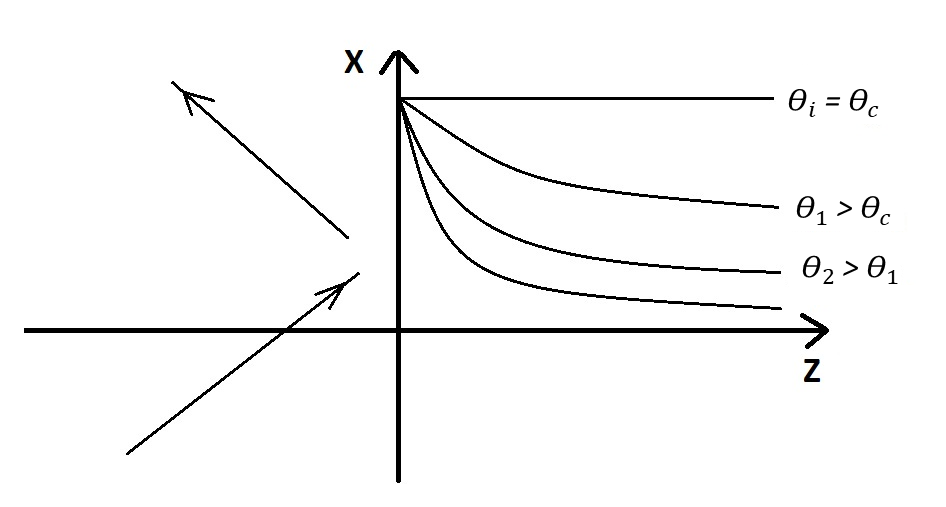
\includegraphics[width=1\linewidth]{\pathtopartone/graphics/amplitude_decay2}
\caption{Graph of incidence and reflection}
\end{figure}

For fields in medium 1;
\begin{equation}
E_i = E_i e^{- j \beta_1(x\sin\theta_i + z\cos\theta_i)}
\end{equation}
\begin{equation}
E_r = E_r e^{- j \beta_1(x\sin\theta_i - z\cos\theta_i)}
\end{equation}
So the total electric field in medium 1 is given as;
\begin{equation*}
E = E_i + E_r
\end{equation*}
\begin{equation*}
E =  E_i e^{- j \beta_1(x\sin\theta_i + z\cos\theta_i)} + E_r e^{- j \beta_1(x\sin\theta_i - z\cos\theta_i)}
\end{equation*}
Since the magnitude of the reflection coefficient is $1$,  $|E_{i}|$ = $|E_{r}|$ but with a phase difference. So we can say that, $E_{r} = E_{i}e^{j\phi}$.
Hence,
\begin{equation*}
E = E_i e^{- j \beta_1x\sin\theta_i}\{ e^{- j \beta_1z\cos\theta_i} + e^{j \phi}
e^{j \beta_1 z\cos\theta_i} \}
\end{equation*}

Depending on the phase difference $\phi$, the term $e^{- j \beta_1z\cos\theta_i} + e^{j \phi}
e^{j \beta_1 z\cos\theta_i}$ is always going to create a constructive or destructive interference in the z-direction. While the term $ e^{- j \beta_1x\sin\theta_i}$ gives a travelling wave in the x direction.

So in medium 1 from the equation, we have a fully developed standing wave in the z direction but a travelling wave in the x direction. In medium 2 it was an exponentially decaying field and a travelling wave in the x direction with the same phase constant as in medium 1 travelling wave in the x direction. Now we can then plot the fields in the two media depending upon the phase of reflection $\phi$, so the field distribution is like a corrugated surface in medium 1 and a decaying field in medium 2. The constant phase plane is determined by $e^{- j \beta_{1}x\sin\theta_i}$. So the constant phase plane is the yz plane. The constant amplitude plane is in the xy plane. So this complex amplitude distribution of the wave travels in the x direction with a phase constant $\beta_1\sin\theta_i$.
\begin{figure}[h]
\centering
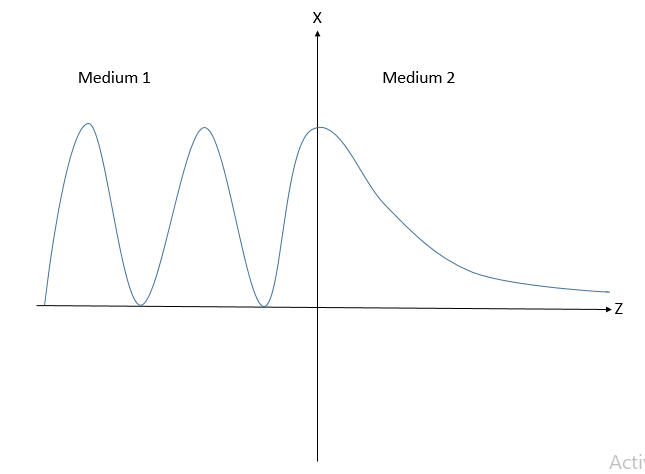
\includegraphics[width=1\linewidth]{\pathtopartone/graphics/mediumplane}
\caption{Graph of field distribution}
\label{fig:mediumplane}
\end{figure}

So whenever total internal reflection occurs, you have this complex distribution of amplitude in space, one side exponentially decaying fields, the other side standing wave kind of fields. This amplitude distribution travels in the x direction with a phase velocity in the x direction $v_{px} = \frac{\omega}{\beta_1\sin\theta_i}$.

Now we may ask, \emph{what is the direction of net power flow?} The fields in medium 2 do not constitute any wave, so no power flow in the z-direction. With no power flow in the z direction in medium 2, there can be no power flow in the z direction in medium 1 also. Since if the power had come from medium 1 in the z direction, and the power can't flow in medium 2, the interface does not consume power since we are talking of a completely lossless medium. Hence whatever power came from the medium 1 incident on the boundary, essentially gets reflected back to give the standing wave shown in medium 1. This implies that there is no power flow perpendicular to the interface but there is a power flow along the interface since we have a travelling wave in the x direction. So when the total internal reflection phenomenon takes place, the net power flow\index{net power flow} is along the interface or in other words, the dielectric interface is capable of guiding electromagnetic energy.

\section{Wave Guides}\index{wave guides}

So we can make use of a dielectric interface for guiding electromagnetic energy along a path. Precisely this is what is used in structures called WAVEGUIDES, and especially when we talk about dielectric media this is what happens in optical fibres. An optical fibre is nothing but a structure having a dielectric interface. So with a wave launched at an angle $\theta_i > \theta_c$,
then there is a total internal reflection in medium 1. The field in medium 2 will exponentially decay. Power flow will be along the interface.

\begin{figure}[h]
\centering
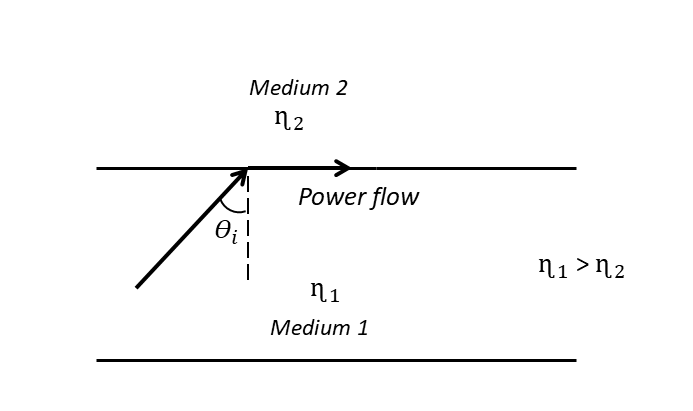
\includegraphics[width=1\linewidth]{\pathtopartone/graphics/optical_fibre}
\caption{Power flow in optical fibre structure}
\label{fig:optical_fibre}
\end{figure}

So if we create some structure like this, it can carry electromagnetic energy over a long distance without any loss as such. Energy is confined in the region of $n_1$ and it will propagate along the interface as a result of total internal reflection. So total internal reflection has played an important role in modern optical communication and helped in the design of structures called optical fibres. 


\begin{mdframed}[ backgroundcolor=lightblue, linewidth=1pt, hidealllines=true]
\section{Exercises:}
\begin{ExerciseList}
\Exercise[label={ex321}]
Describe the mathematical conditions necessary for total internal reflection and explain the critical angle's role.
\Exercise[label={ex322}]
Derive the reflection coefficients for both perpendicular and parallel polarizations in total internal reflection.
\Exercise[label={ex323}]
How do phase changes differ between parallel and perpendicular polarizations during total internal reflection? Explain with equations.
\Exercise[label={ex324}]
Analyze the behavior of fields in medium 2 during total internal reflection and discuss their impact on the phenomenon.
\Exercise[label={ex325}]
Define reactive fields and their relationship to power flow in the context of total internal reflection. Provide examples.
\Exercise[label={ex326}]
Discuss the role of Snell's Law in determining the possibility of total internal reflection and its significance.
\Exercise[label={ex327}]
Compare and contrast the amplitude and phase distributions of waves in medium 1 and medium 2 during total internal reflection.
\Exercise[label={ex328}]
Explain the critical angle's significance in determining the behavior of transmitted waves during total internal reflection.
\Exercise[label={ex329}]
How does total internal reflection facilitate the guiding of electromagnetic energy in wave guides such as optical fibers? Discuss its practical applications.
\Exercise[label={ex3210}]
Analyze the phase velocity in the x-direction and power flow along the interface during total internal reflection, elaborating on their relationships and implications.
\end{ExerciseList}
\end{mdframed}
